\section{Appendices}
%%%%%%%%%%%%%%%
%							SUPERVISOR MEETINGS
%%%%%%%%%%%%%%%
\subsection{Semester 2 Supervisor Meetings}

\begin{table}[H]
	\centering
	\begin{tabular}{|l|l|l|}
		\hline
		\multicolumn{3}{|c|}{\textbf{2017 Supervisor Meeting Summary}}                                                                                                                                                                                                                              \\ \hline
		\textit{Date} & \textit{Time} & \textit{Discussion Points}                                                                                                                                                                                                                                  \\ \hline
		31 Jan 2017   & 1200-1230     & \begin{tabular}[c]{@{}l@{}}- Feedback from 2016 reports\\ - Research shortcomings\\ \\ - My plan for remaining tasks\\ - Explained where I was wrong with terminology\end{tabular}                                                                          \\ \hline
		17 Apr 2017   & 1300-1400     & \begin{tabular}[c]{@{}l@{}}- Report structure changes\\ - Different PV calculation techniques\\ - Necessary additions to PV section\\ - Incorrect assumptions during calculation\\ - Discussed remaining tasks\\ - Discussed oral presentation\end{tabular} \\ \hline
	\end{tabular}
	\caption{Supervisor Meetings of 2017 Summary}
	\label{table:supervisor-meeting-summary}
\end{table}

\newpage

%%%%%%%%%%%%%%%
%							TIMELINE
%%%%%%%%%%%%%%%

\subsection{Timeline Analysis} \label{appendix:Timeline}

\paragraph{}
The tasks were be split into days and University weeks. It was ensured to include the holidays during periods where University is not run. This project does not simply end upon the completion of this semester. BEB801 is concluded on November 4th at the end of Week 14, however BEB802 is the subject allocation to complete the second half of this project. The task table will allocate SMART milestones. Additionally, the benefits of completing the subjects during this period is that there is the additional time from summer holidays to account for.

\paragraph{}
Table \ref{table:timeline_original} on the following page shows the milestones of this project. The University assigned submissions are represented as bold text. The four major deliverables for the first half of this project are the library assessment, project proposal, oral presentation and progress report. These four deliverables are what have outlined how the remaining tasks have been created and the time periods allowed for. Earlier due dates are set to allow for editing or possible difficulties to occur without major repercussions. 

\paragraph{}
Table \ref{table:timeline_revised} represents the revised timeline with completed times. This is for the benefit of both the creator of this project as well as any future students who wish to progress the project and extend its scope. There are a variety of reasons as to why there were extensions of time for completing milestones. It is not an irregular occurrence that project plans are extended and this project is no different. As previously discussed, deadlines were set at least 1 week early with the intention of ensuring proper preparation is done and deadlines are not missed.     

\newpage
\textbf{Initial Timeline}

% Table of Tasks
\begin{table}[H]
	\centering
	\begin{tabular}{||c c||} 
		\hline
		\multicolumn{2}{|c|}{\textbf{Initial Project Timeline}} \\ [0.5ex] 
		\hline\hline
		\textbf{Milestone} & \textbf{Deadline} \\ 
		\hline\hline
		Project Definition 							& Sem 1 Week 3 \\ 
		\textbf{Library Assessment} 				& \textbf{Sem 1 Week 4} \\
		Initial Research Phase 						& Sem 1 Week 6 \\
		\textbf{Project Proposal} 					& \textbf{Sem 1 Week 7} \\
		Initial Design Phase 						& Sem 1 Week 9 \\
		Initial Prototype Design Finalised 			& Sem 1 Week 11 \\
		Initial 3D Modelling for Presentation 		& Sem 1 Week 12 \\
		\textbf{Initial Oral Presentation} 			& \textbf{Sem 1 Week 14} \\ 
		\textbf{Written Report} 					& \textbf{Sem 1 Week 14} \\ 
		Implement Feedback From Report 				& Summer Break \\
		Complete Research Shortcomings 				& Summer Break \\
		Complete Further Technical Calculations 	& Summer Break \\
		Initial Finance Analysis 					& Sem 2 Week 2 \\
		Design Simulations 							& Sem 2 Week 6 \\
		\textbf{Progress Report} 					& \textbf{Sem 2 Week 7} \\
		Finalised Design 							& Sem 2 Week 10 \\
		Finalised Simulations \& 3D Modelling 		& Sem 2 Week 11 \\
		Finalised Financial Analysis				& Sem 2 Week 12 \\
		\textbf{Final Presentation} 				& \textbf{Sem 2 Week 14} \\
		\textbf{Final Report} 						& \textbf{Sem 2 Week 14} \\ [1ex] 
		\hline
	\end{tabular}
	\caption{Initial Project Timeline}
	\label{table:timeline_original}
\end{table}    

\newpage
\textbf{Revised Timeline}

% Table of Tasks
\begin{table}[H]
	\centering
	\begin{tabular}{||p{5cm} c c||} 
		\hline
		\textbf{Milestone} & \textbf{Original Deadline} & \textbf{Actual Completion} \\ [0.5ex] 
		\hline\hline
		Project Definition 							& Week 3 			& Week 3\\ 
		\textbf{Library Assessment} 				& \textbf{Week 4} 	& Week 4\\
		Initial Research Phase 						& Week 6 			& Week 6\\
		\textbf{Project Proposal} 					& \textbf{Week 7} 	& Week 7\\
		Initial Design Phase 						& Week 9			& Week 10\\
		Initial Prototype Design Finalised 			& Week 11 			& NA\\
		Initial 3D Modelling for Presentation 		& Week 12 			& Week 11\\ 
		\textbf{Initial Oral Presentation} 			& \textbf{Week 14} 	& Week 14\\
		\textbf{Written Report} 					& \textbf{Week 14} 	& Week 14\\ 
		Implement Feedback From Report 				& Summer Break 		& Summer Break \\
		Complete Research Shortcomings 				& Summer Break 		& Summer Break \\
		Complete Further Technical Calculations 	& Summer Break 		& Week 8 \\
		Initial Finance Analysis 					& Week 2 			& TBC \\
		Design Simulations 							& Week 6 			& Week 8 \\ 
		\textbf{Progress Report} 					& \textbf{Week 8} 	& Week 8 \\
		Finalised Design 							& Week 10 			& TBC \\
		Finalised Simulations \& 3D Modelling 		& Week 11 			& TBC \\
		Finalised Financial Analysis 				& Week 12 			& TBC \\ 
		\textbf{Final Presentation} 				& \textbf{Week 14} 	& TBC\\
		\textbf{Final Report} 						& \textbf{Week 14} 	& TBC\\ [1ex] 
		\hline
	\end{tabular}
	\caption{Initial Project Timeline Analysis}
	\label{table:timeline_revised}
\end{table}      



%%%%%%%%%%%%%%%
%							LEVEL 6 MARKUP
%%%%%%%%%%%%%%%
\newpage
\subsection{QUT P Block Level 6 Office Markup}
\label{appendix:qut_lvl6_markup}
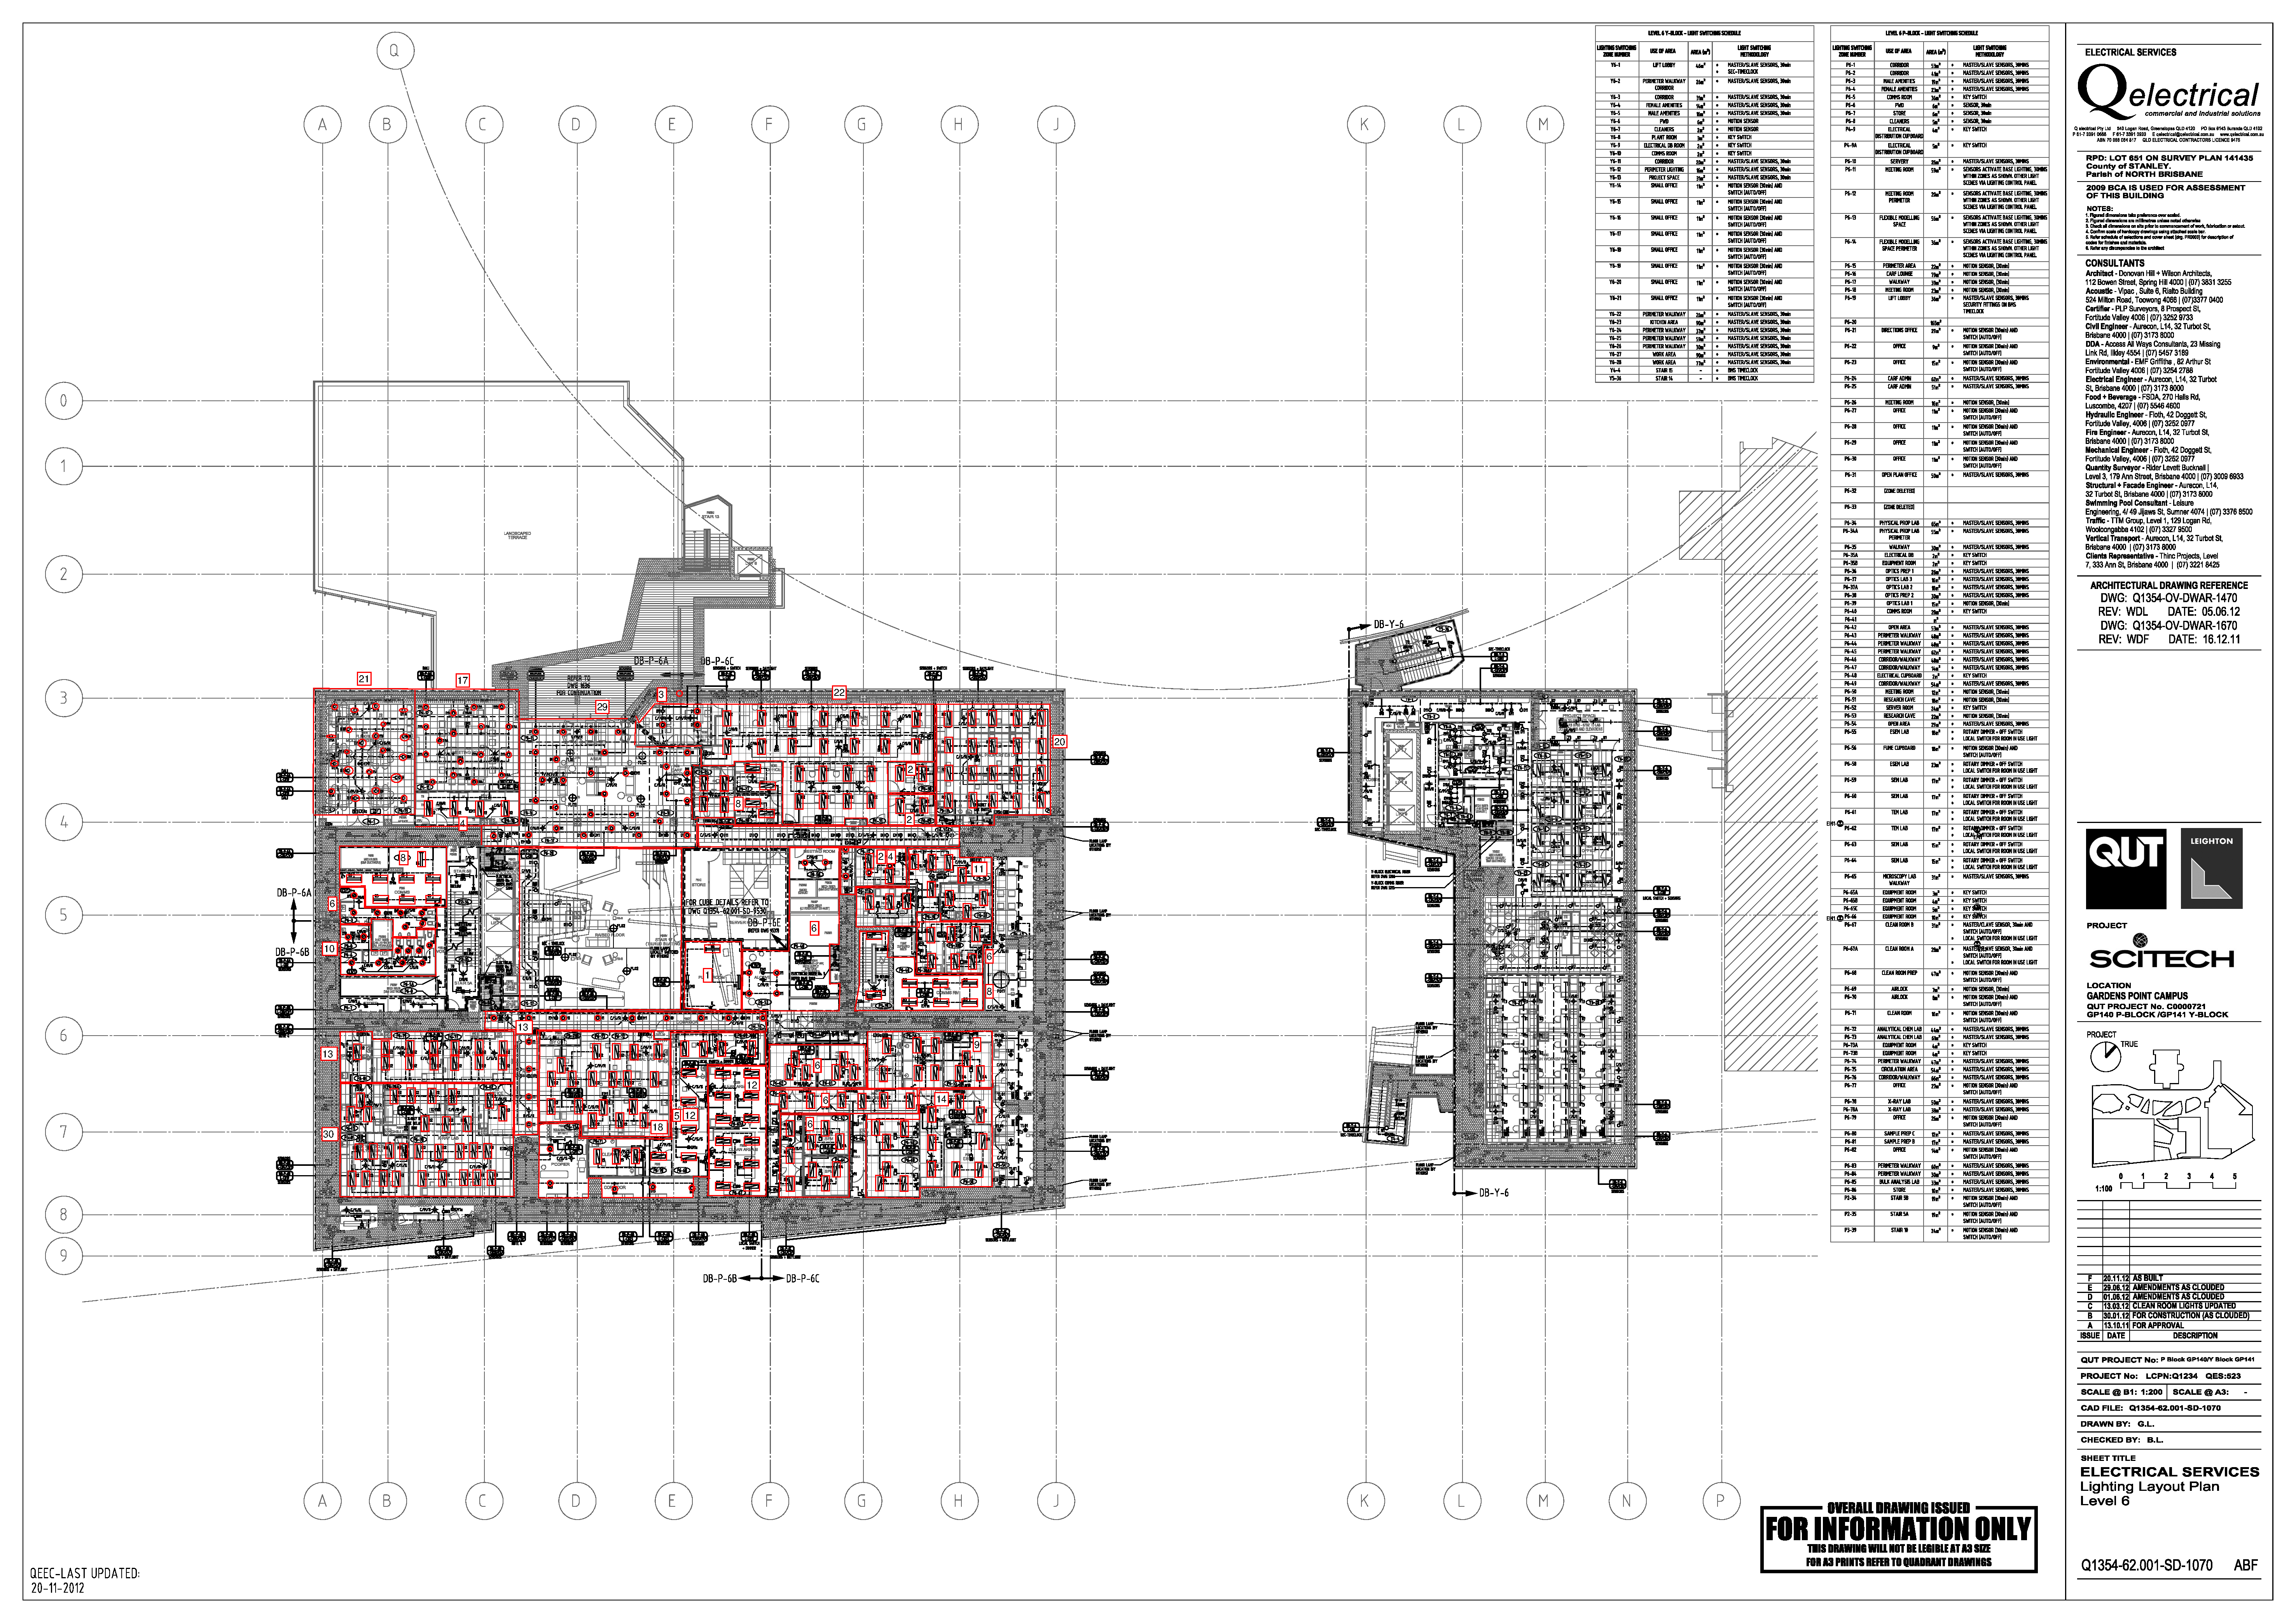
\includepdf[pages={1},angle=-90]{appendix/qut_lvl6_markup}

%%%%%%%%%%%%%%%
%							LEVEL 6 OFFICE LIGHITNG SIMULATION
%%%%%%%%%%%%%%%

\subsection{QUT P Block Level 6 Office Lighting Simulation}
\label{appendix:QUT-Lvl6-office-rev3}
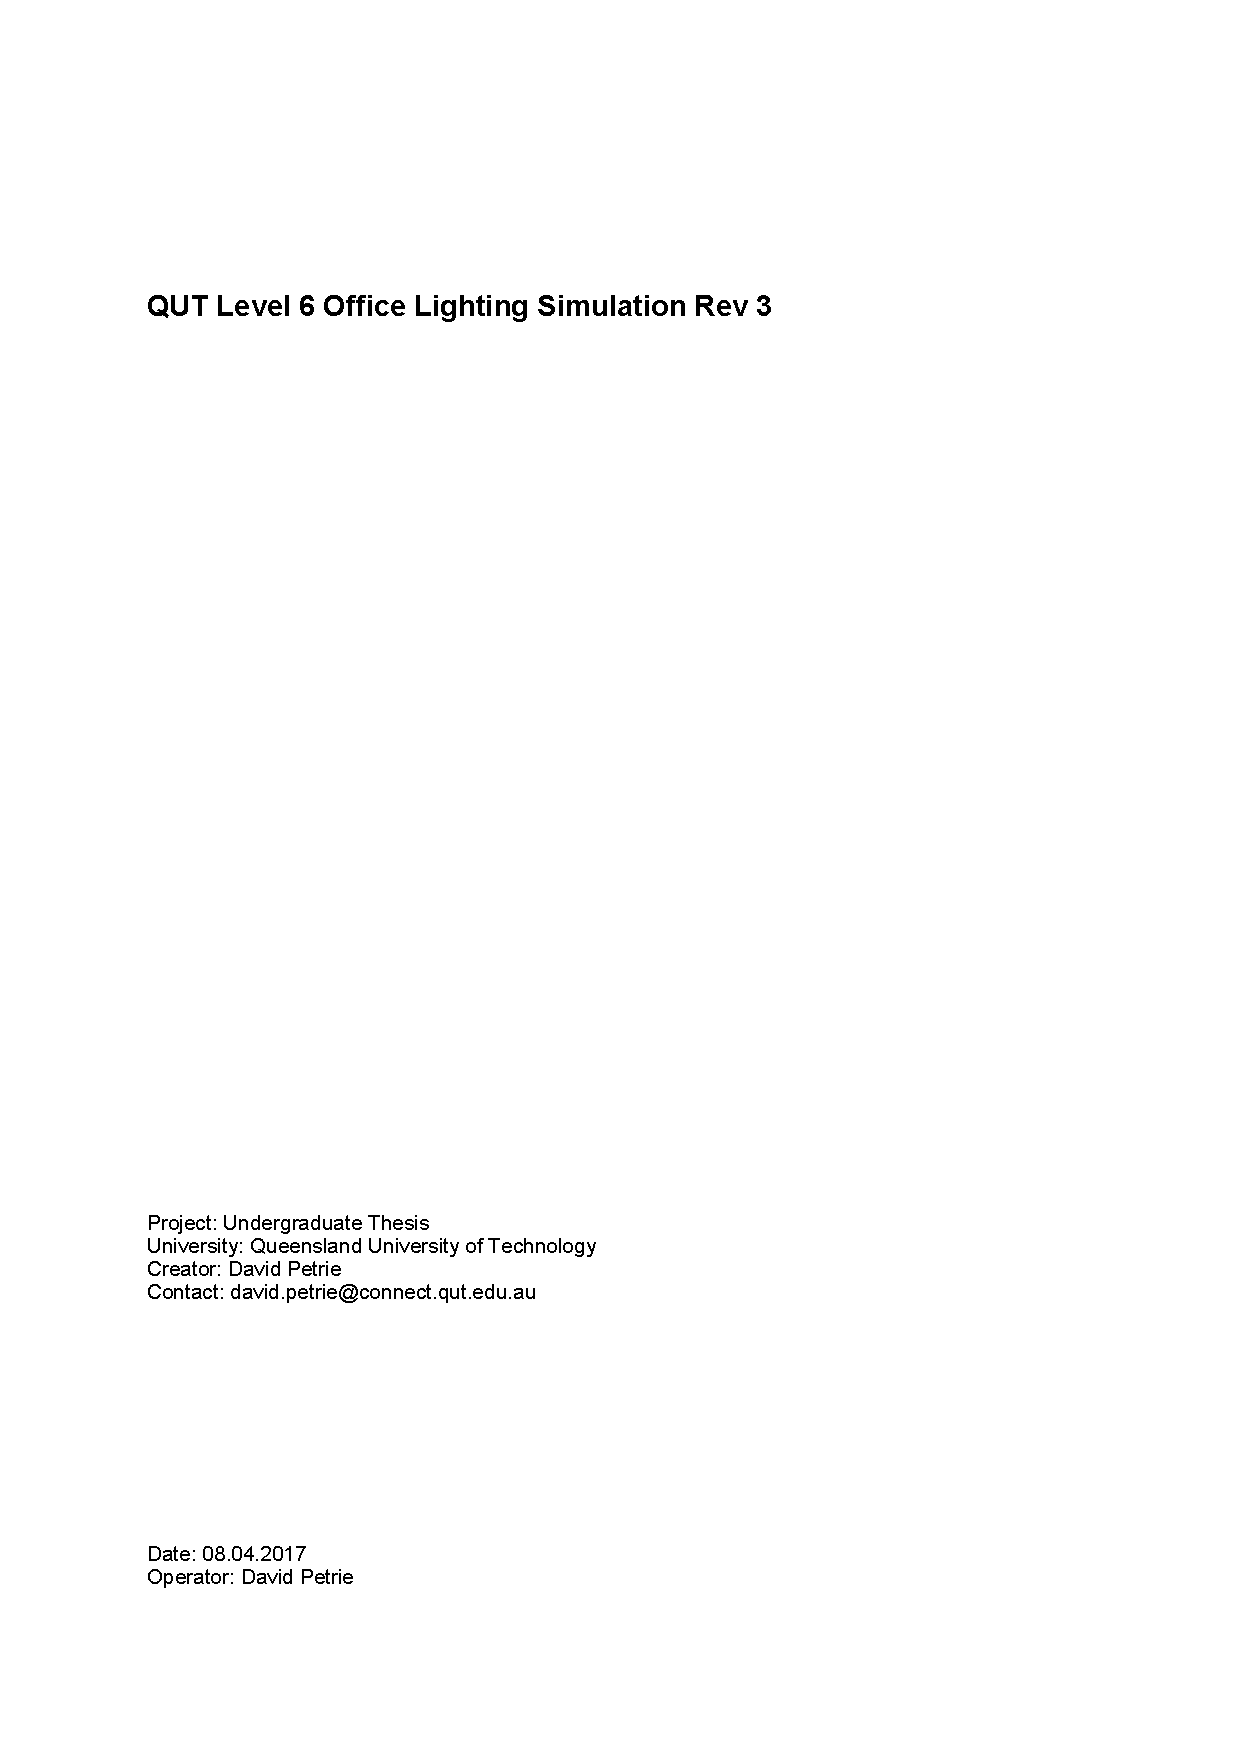
\includepdf[pages={1-8}]{appendix/QUT-Lvl6-office-rev3.pdf}

%%%%%%%%%%%%%%%
%							DRAFT FLOORPLAN DIALUX REPORT
%%%%%%%%%%%%%%%

\subsection{Draft Floor Plan Lighting Analysis Report}
\label{appenddix:DraftFloorPlanLighting}
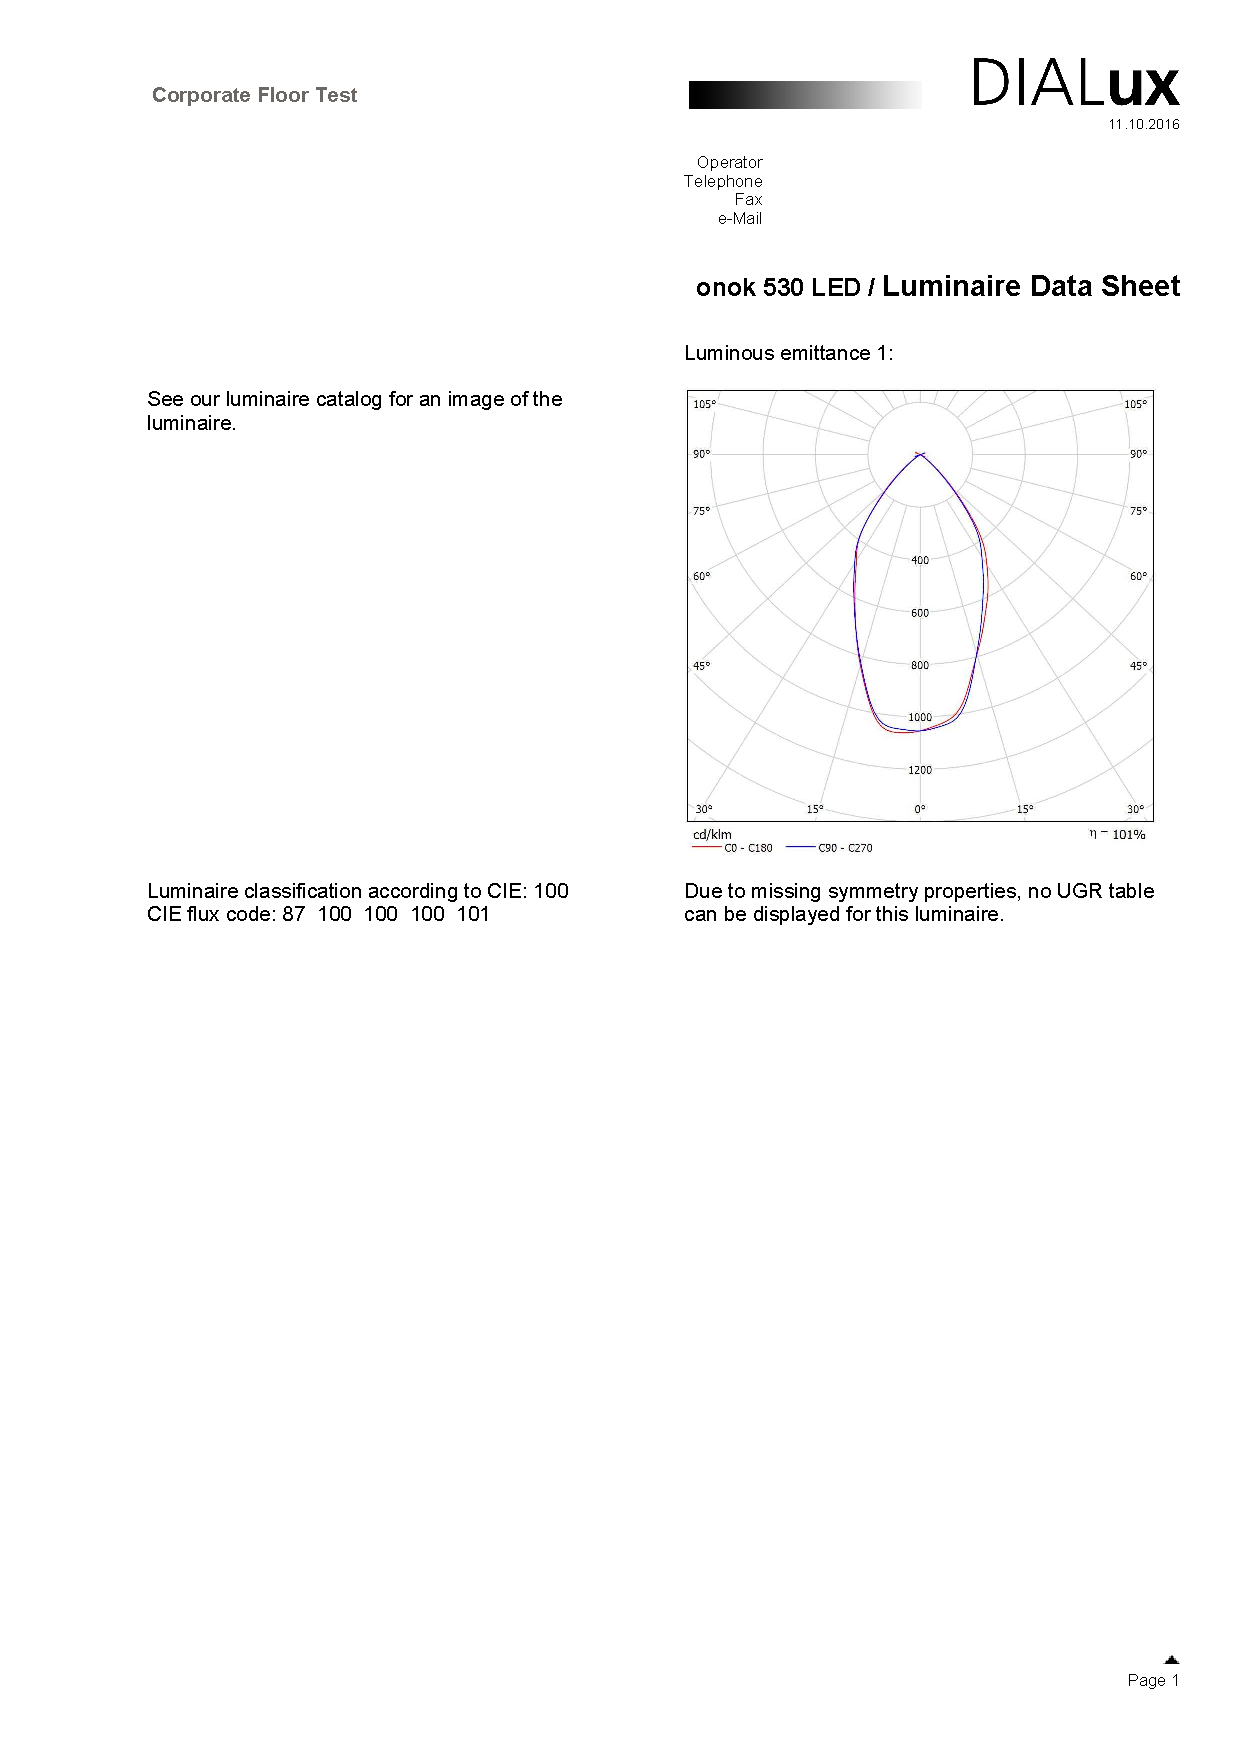
\includepdf[pages={1-12}]{appendix/draft_light_report.pdf}


